%!TEX root = draft.tex

% datasets table..
\begin{table*}[b]
 {
  \begin{tabular}[c]{llrrrc|rrrr} \toprule
   Network &  Description & $|V|$           & $|E|$        & $T$        & $A$, $|A|$  &  \texttt{LN} $(\mu, \sigma)$ & \texttt{DPL} $\alpha$       &  Avg. ${\texttt{LCC}}$  & \texttt{AA} $r$           \\ \midrule
   \texttt{USSC}~\cite{fowler2008authority}  & U.S. Supreme Court cases         & 30,288     & 216,738      & 1754-2002  & -   & (1.19, 1.18) & 2.32     & 0.12    & -     \\
   \texttt{HEP-PH}~\cite{gehrke2003overview} & ArXiv Physics manuscripts     & 34,546     & 421,533      & 1992-2002  & -  &   (1.32, 1.41) & 1.67     & 0.12    & -                 \\
   \texttt{Semantic}~\cite{ammar}&   Academic Search Engine  & 7,706,506  & 59,079,055   & 1991-2016  & -   &   (1.78, 0.96)  & 1.58     & 0.06    & -             \\   \midrule
   \texttt{ACL}~\cite{acldata}    & NLP papers      & 18,665     & 115,311      & 1965-2016  & \textsc{venue}, 50  &   (1.93, 1.38)  & 1.43     & 0.07    & 0.07  \\
   \texttt{APS}~\cite{aps}     & Physics journals     & 577,046    & 6,967,873    & 1893-2015  & \textsc{journal}, 13 &   (1.62, 1.20)  & 1.26     & 0.11    & 0.44 \\
   \texttt{Patents}~\cite{leskovec2005graphs}   & U.S. NBER patents    & 3,923,922  & 16,522,438   & 1975-1999  & \textsc{category}, 6 &   (1.10, 1.01)   & 1.94     & 0.04    & 0.72 \\
   % \texttt{PYPI}         & 25,169     & 71,371       & 2002-2018  & \textsc{category} & 9  \\
  \bottomrule
  \end{tabular}
  \vspace{1mm}
  \caption{Summary statistics \& global properties of six network datasets: $|V|$ nodes join the networks and form edges $|E|$ over
  time period $T$. In attributed networks, each node has a categorical attribute value that belongs to set $A$ of size $|A|$.
  The networks exhibit lognormal (\texttt{LN}) in-degree distribution with mean $\mu$ and standard deviation $\sigma$,
  high average local clustering (${\texttt{LCC}}$) \& attribute assortativity (\texttt{AA}) coefficient and
  densify over time with power law (\texttt{DPL}) exponent $\alpha$.}
  \label{table:datasets}
  \label{table:netstats}
 }
\end{table*}


\section{Introduction}
\label{sec:Introduction}


% what is the problem?

We present a network growth model that explains how distinct
structural properties of attributed networks can emerge from local edge
formation processes. In real-world networks, individuals tend to form edges
under resource constraints such as limited information and partial network access.
Additionally, phenomena such as triadic closure and homophily
\textit{simultaneously} influence individuals' decisions to form connections.
Over time, these decisions cumulatively shape real-world networks to exhibit
rich structural characteristics: heavy-tailed in-degree distribution, skewed
local clustering and homophilic mixing patterns. However, we lack an
understanding of local, resource constrained mechanisms that incorporate
sociological factors to explain the emergence of these rich structural
characteristics over time.

% The problem of developing a model of network growth, where individuals act under
% resource constraints, including access to only local information is hard. The
% problem lies in identifying simple mechanisms with few parameters that unifies
% multiple sociological phenomena to \textit{jointly} preserve structural
% properties and attribute mixing patterns of attributed networks.

% on edge formation as well as preserve global network structure.

% why is it important?

Classic models of network growth tend to make unrealistic assumptions about how
individuals form edges. Consider a simple stylized example: the process of
finding a set of papers to cite when writing an article. In preferential
attachment \cite{barabasi1999emergence} or fitness
\cite{bianconi2001bose,caldarelli2002scale,wang2013quantifying} based models, a
node making $m$ citations would pick papers from the \textit{entire} network in
proportion to their in-degree or fitness respectively. This process assumes that
individuals possess {complete} knowledge of in-degree or fitness of every node
in the network. An equivalent formulation---vertex copying
\cite{kumar2000stochastic}---induces preferential attachment: for every
citation, a node would pick a paper uniformly at random from \textit{all}
papers, and either cite it or copy its citations. Notice that the copying
mechanism assumes individuals have complete access to the network and forms each
edge independently. Although these models explain the emergence of power law
degree distributions, they are unrealistic: they require global knowledge (e.g.,
preferential attachment requires knowledge of the global in-degree distribution)
or global access (e.g., vertex copying requires random access to all nodes).
Moreover, these models do not account for the fact that many
networks are attributed (e.g., a paper is published at a venue; a Facebook user
may use gender, political interests to describe them) and that assortative
mixing is an important network characteristic~\cite{newman2002assortative}.

Recent papers tackle resource constraints \cite{mossa2002truncation,zeng2005construction,wang2009local} as well as nodal attributes
\cite{de2013scale,gong2012evolution}. However, the former disregard attributes and the latter do not provide a realistic representation
of edge formation under resource constraints. Furthermore, both sets of models do not preserve multiple structural properties jointly and accurately.
Developing a parsimonious and accurate model of attributed network growth that accounts for observed
sociological phenomena is non-trivial. Accurate network growth models are useful
for synthesizing networks as well as to extrapolate existing real-world networks.

% representations of how individuals make decisions about edge formation. A
% realistic representation of how individuals form edges necessitates modeling the
% effect of multiple sociological phenomena on edge formation under resource
% constraints.

%why is it hard?


% what did we do?
\begin{figure}[t]
	\centering
	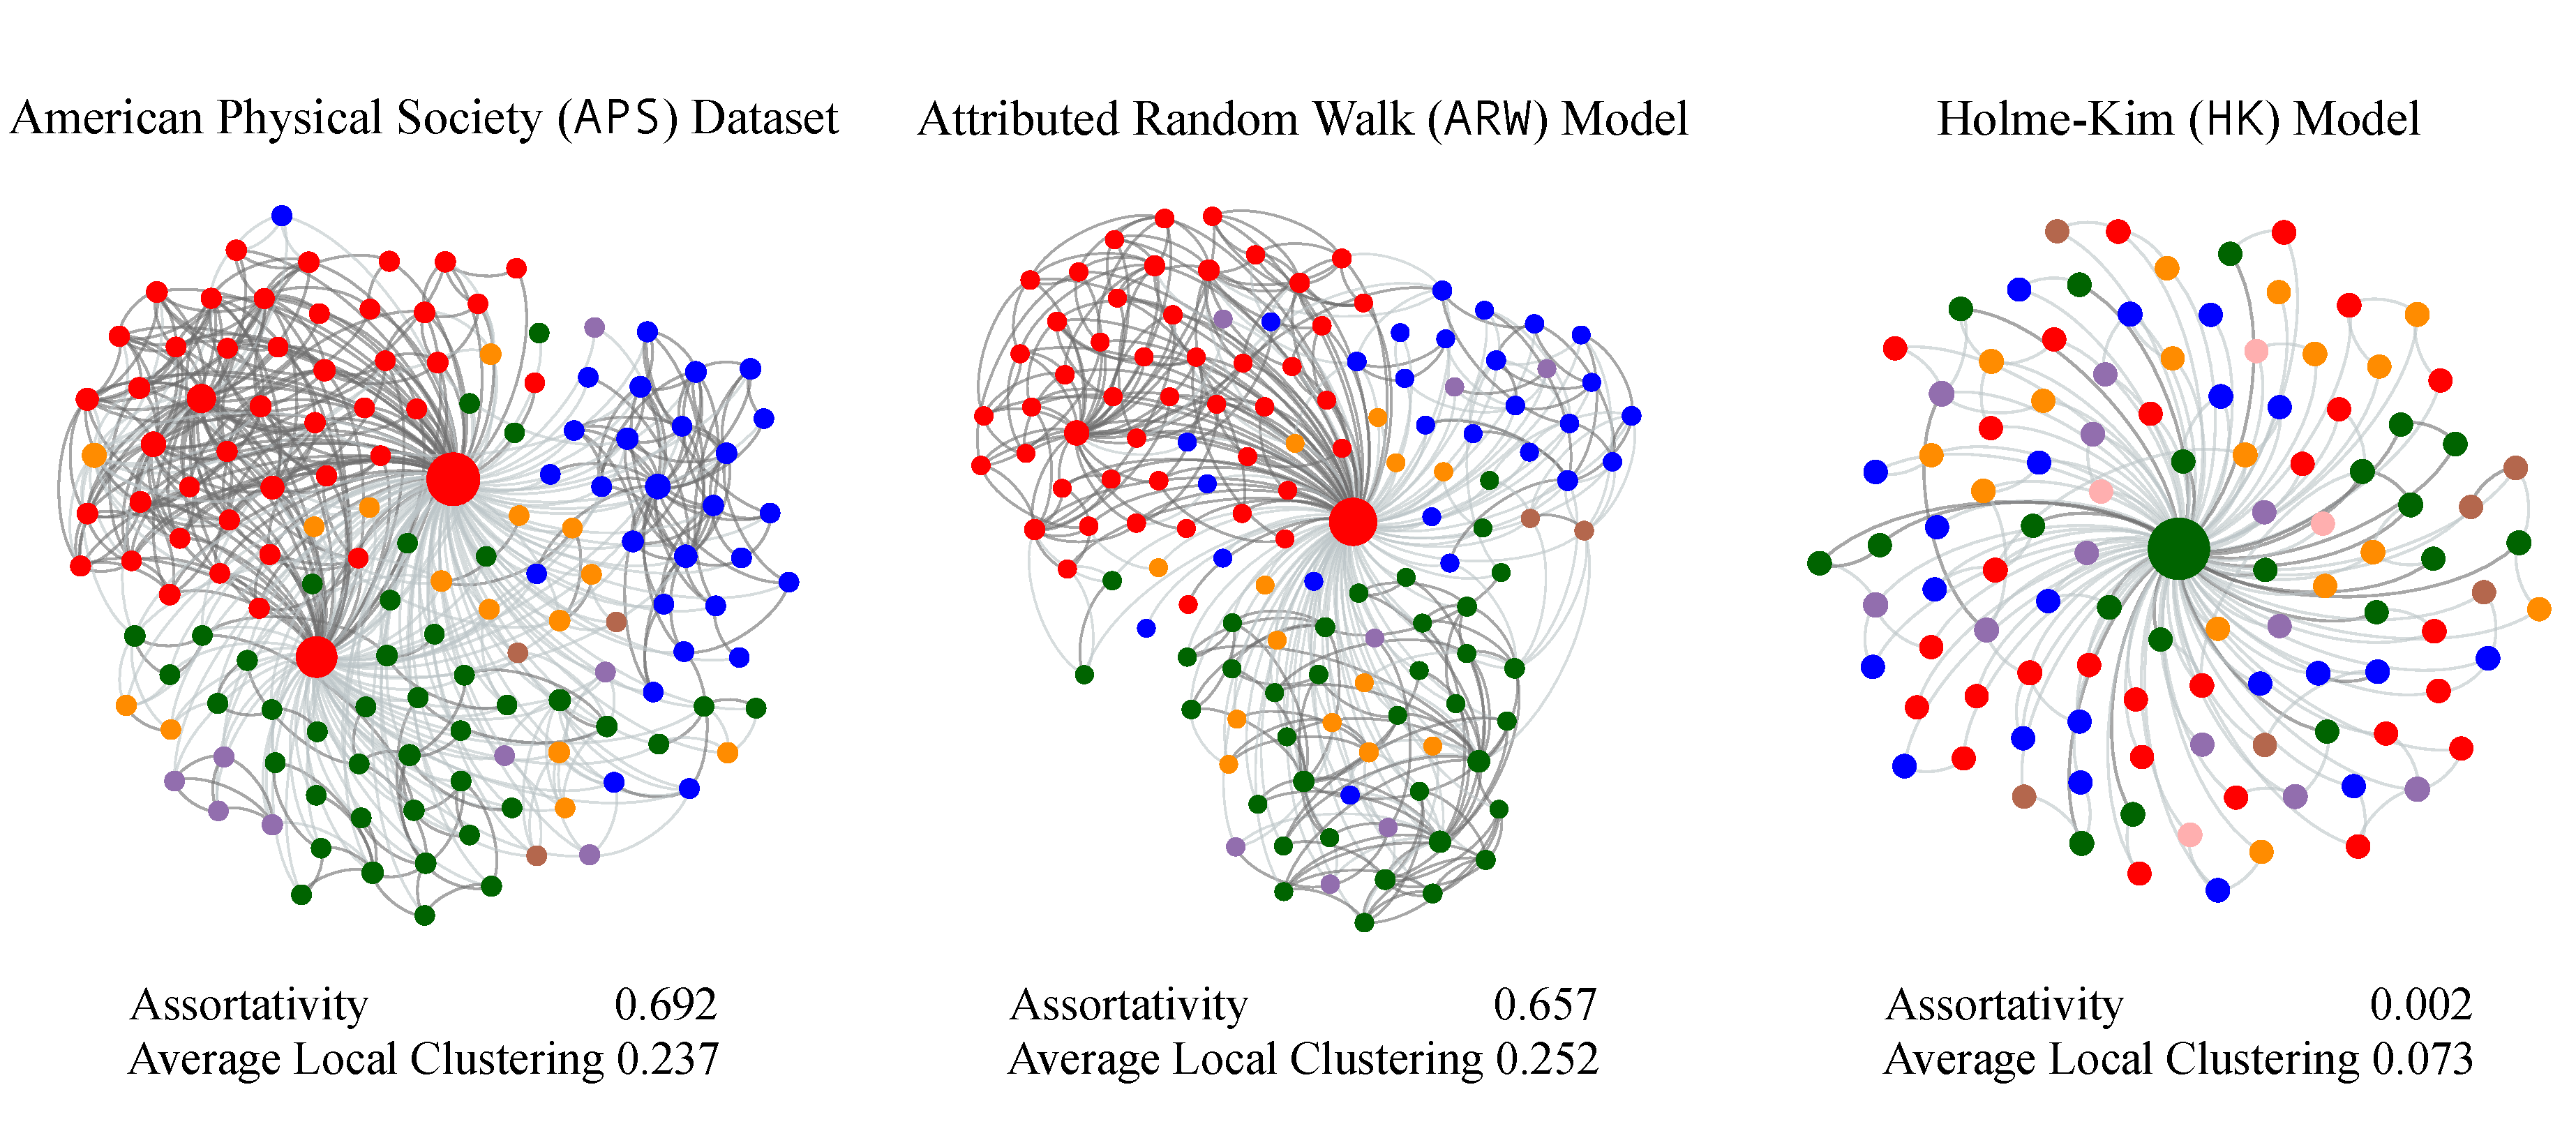
\includegraphics[width=\columnwidth]{experiments_final4}
	\caption{The figure shows how our proposed model of an Attributed Random Walk (\texttt{ARW}) accurately preserves local clustering and assortativity; we contrast with a non-attributed growth model~\cite{holme2002growing} to underscore the importance of using attributes for network growth.}
	\label{fig:intro_plot}
\end{figure}


We propose an Attributed Random Walk (\texttt{ARW}) model that jointly explains
the emergence of in-degree distributions, local clustering, clustering-degree
relationship and attribute mixing patterns through a resource constrained mechanism based on random walks (see~\Cref{fig:intro_plot}). In particular, \texttt{ARW} relies entirely on local information to grow the network, without access to information of all nodes. In \texttt{ARW}, incoming nodes select a seed node based on attribute similarity and initiate a biased random walk: at each step of the walk, the incoming node either jumps back to its seed or chooses an outgoing link or incoming link to visit another node; it links to each visited node with some probability and halts after it has exhausted its budget to form connections. We have three primary contributions:
\begin{enumerate}
\item \textbf{Attributed:} We propose a parsimonious and accurate model of attributed network growth.
\item \textbf{Local information:} Our model is based on a random walk and uses local processes to form edges, without recourse to global information of the network.
\item \textbf{Unified account:} To the best of our knowledge, \texttt{ARW} is the first model that accounts for multiple sociological phenomena---bounded rationality; structural constraints; triadic closure; attribute homophily; preferential attachment---through an entirely local process to model global network structure and attribute mixing patterns.
\end{enumerate}



% We conducted extensive experimental results against state-of-the-art
% baselines on large and diverse citation network datasets.
% We focus on directed citation networks
%  in this paper, as these networks---where all node edges form at the time of node joining---offer a clean foundation to explain growth in social networks (e.g. via a ``pause \& restart'' parameter), where edges can form after a node joins.
\texttt{ARW} preserves
multiple structural properties---in-degree distribution, clustering and
in-degree \&clustering relationship---with high accuracy.
Our experiments on six large-scale network datasets indicate that the proposed growth model outperforms
eight state-of-the-art network growth models, including attributed growth models, by a
statistically significant margin of 2.5--$10\times$.

The rest of the paper is organized as follows.
We begin by defining the problem statement in~\Cref{sec:Problem Statement}.
In~\Cref{sec:Analysis}, we outline six network datasets, describe key structural
properties of real-world networks and discuss insights from sociological studies.
Then, in~\Cref{sec:Proposed Model}, we describe the network growth model. We follow
by presenting experiments in ~\Cref{sec:Experiments}, analysis of assortative mixing
in ~\Cref{subsec:LocalMixing} and discussion in~\Cref{sec:Discussion}.
We conclude in~\Cref{sec:Conclusion}.

% In~\Cref{sec:Related Work}, we
% describe the related work. Then, in~\Cref{sec:Preliminaries}, we define key
% structural properties and introduce the datasets. We formally state the goal of
% the paper in~\Cref{sec:Problem Statement}. In~\Cref{sec:Empirical Analysis}
% and~\Cref{sec:Proposed Model}, we report prominent structural characteristics
% of citation networks and propose a network growth model respectively. This is
% followed by~\Cref{sec:Experiments}, where we validate our model against
% multiple baselines.